\begin{tikzpicture}
\node[inner sep=0,anchor=south west] (im) at (0,0) {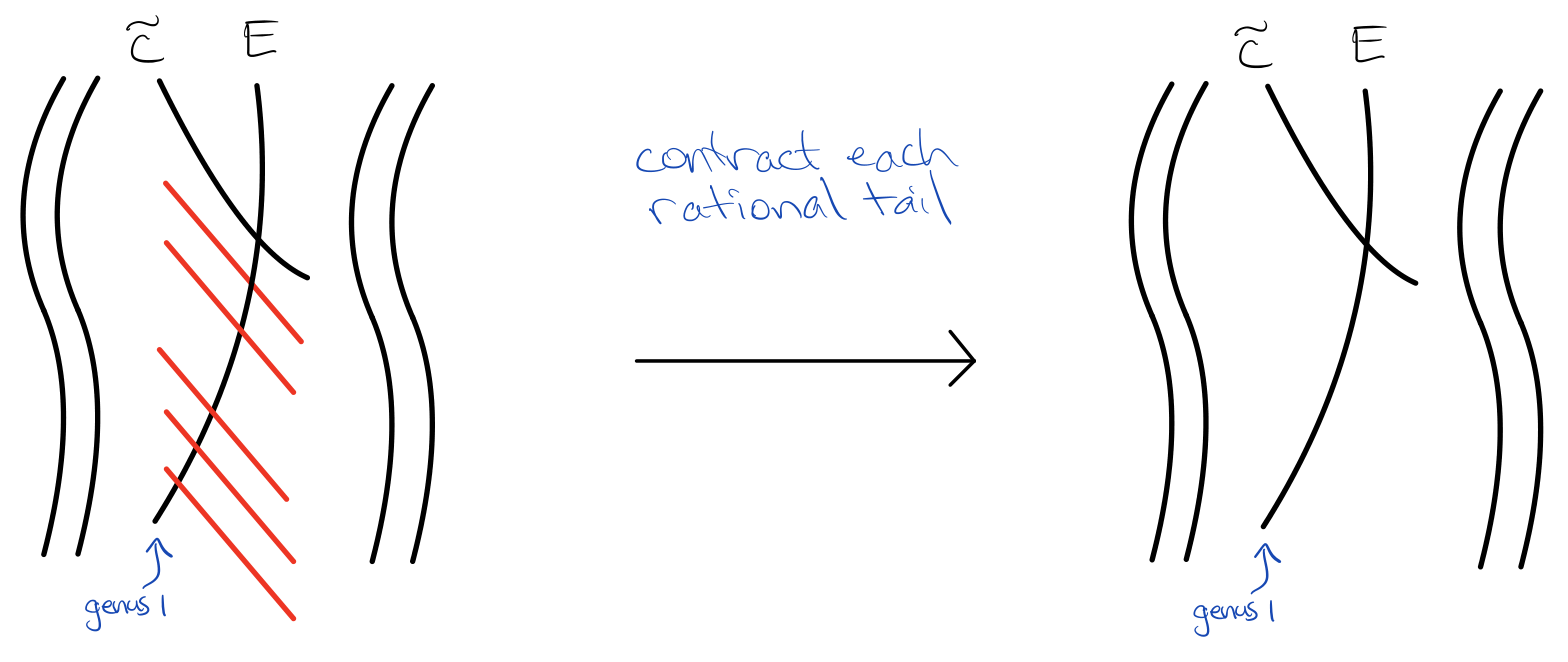
\includegraphics[width=.86\textwidth]{figures/reduction-step6.png}};
\begin{scope}[x={(im.south east)},y={(im.north west)}]
\fill[white] (0.37,0.62) rectangle (0.64,0.86);
\fill[white] (0.045,0.005) rectangle (0.13,0.085);
\fill[white] (0.75,0.005) rectangle (0.83,0.085);
\node[fill=white,inner sep=1pt,font=\scriptsize,text=blue] at (0.51,0.79) {收缩每条};
\node[fill=white,inner sep=1pt,font=\scriptsize,text=blue] at (0.51,0.7) {有理尾};
\node[fill=white,inner sep=1pt,font=\scriptsize,text=blue] at (0.085,0.055) {亏格 $1$};
\node[fill=white,inner sep=1pt,font=\scriptsize,text=blue] at (0.8,0.055) {亏格 $1$};
\end{scope}\end{tikzpicture}
